% =====================================================================
%  Query lifecycle (vertical flowchart), after [L14, s.5]
%  Compile:  pdflatex query-lifecycle.tex   (inside this folder)
%  Output:   query-lifecycle.pdf  -> 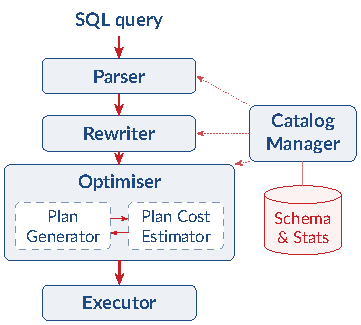
\includegraphics{query-lifecycle}
% =====================================================================
\makeatletter\def\input@path{{../../theme/}}\makeatother   % shared palette
\documentclass[tikz,border=2pt,11pt]{standalone}
\usepackage[T1]{fontenc}
\usepackage[defaultsans]{lato}
\renewcommand{\familydefault}{\sfdefault}
\usepackage{vinuni-palette}
\usetikzlibrary{positioning,arrows.meta,shapes.geometric,fit,backgrounds,calc}

\begin{document}
\begin{tikzpicture}[
    font=\footnotesize, node distance=3.6mm,
    stage/.style={draw=vinuNavy, fill=vinuNavy!8, rounded corners=1mm, minimum width=26mm,
                  minimum height=6mm, text=vinuNavy, font=\footnotesize\bfseries},
    sub/.style={draw=vinuNavy!60, dashed, fill=white, rounded corners=0.8mm, minimum width=16mm,
                minimum height=8mm, align=center, text=vinuNavy, font=\scriptsize},
    flow/.style={-{Stealth[length=1.8mm]}, thick, vinuRed},
    info/.style={-{Stealth[length=1.5mm]}, densely dotted, vinuRed!80}]
  \node[text=vinuNavy, font=\footnotesize\bfseries] (sql) {SQL query};
  \node[stage, below=of sql] (parser) {Parser};
  \node[stage, below=of parser] (rewriter) {Rewriter};
  % Optimiser: container with two sub-components
  \node[sub, below=8.5mm of rewriter, xshift=-9.5mm] (gen) {Plan\\Generator};
  \node[sub, right=3mm of gen] (est) {Plan Cost\\Estimator};
  \draw[-{Stealth[length=1.3mm]}, vinuRed] ([yshift=1.2mm]gen.east) -- ([yshift=1.2mm]est.west);
  \draw[-{Stealth[length=1.3mm]}, vinuRed] ([yshift=-1.2mm]est.west) -- ([yshift=-1.2mm]gen.east);
  \coordinate (optop) at ($(gen.north)+(0,4.5mm)$);   % room for the "Optimiser" label
  \begin{scope}[on background layer]
    \node[draw=vinuNavy, fill=vinuNavy!8, rounded corners=1mm, inner sep=1.8mm,
          fit=(gen)(est)(optop)] (opt) {};
  \end{scope}
  \node[anchor=north, font=\footnotesize\bfseries, text=vinuNavy, inner sep=1pt]
    at ([yshift=-1.2mm]opt.north) {Optimiser};
  \node[stage, below=4mm of opt] (exec) {Executor};
  % main flow
  \draw[flow] (sql) -- (parser);
  \draw[flow] (parser) -- (rewriter);
  \draw[flow] (rewriter) -- (rewriter |- opt.north);
  \draw[flow] (opt.south -| exec) -- (exec);
  % catalog
  \node[stage, right=9mm of rewriter, minimum width=18mm, align=center, font=\footnotesize\bfseries]
    (cat) {Catalog\\Manager};
  \node[cylinder, shape border rotate=90, aspect=0.25, draw=vinuRed, fill=vinuRed!6,
        minimum width=13mm, minimum height=11mm, align=center, text=vinuRed, font=\scriptsize,
        below=4mm of cat] (stats) {Schema\\\& Stats};
  \draw[vinuRed!60] (cat) -- (stats);
  \draw[info] (cat.north west) -- (parser.east);
  \draw[info] (cat.west) -- (rewriter.east);
  \draw[info] (cat.south west) -- (opt.north east);
\end{tikzpicture}
\end{document}
